\section{{\LaTeX}简介}


\begin{WUTquote}{Donald Kunth}
Microsoft Word is the last thing I want to use before I die.
\end{WUTquote}


\par {\LaTeX}是用于产生高品质文档的排版系统,而且事实上已经成为了学术出版的行业标准,国际上绝大多数学术期刊都要求接受{\LaTeX}稿件。{\LaTeX}排版系统基于的是“What you think is what you get.”(所思即所得)的思路\footnote{Microsoft Word、LibreOffice Writer、WPS Writer等排版软件基于的是“What you see is what you get.”(所见即所得)的思路。}。用于只需要关注文档的内容,而计算机会负责相关的格式处理。对于初学者有一定的难度,然而当熟练之后,{\LaTeX}便具有压倒性的优势,尤其是排版大型文档时,比如学位论文或书籍。{\LaTeX}的前身是1978年发布的{\TeX}排版系统,发明人为Donald Kunth教授(图~\ref{fig_Knuth})。1984年,Leslie Lamport博士编写了一组自定义命令宏包,取名LaTeX,该宏包对{\TeX}系统的若干命令进行了重新封装,使得整个排版系统使用起来方便了许多,并于次年发布了LaTeX宏包的源程序。逐渐的,{\TeX}排版系统也就演变为我们今天熟称的{\LaTeX}排版系统。{\LaTeX}是一个开源项目(\url{https://www.latex-project.org/}),世界各地的爱好者为{\LaTeX}系统编写了若干宏包,用于根据用户需求进行各式各样的格式处理,这些宏包及相关的说明文档可以从CTAN网站(Comprehensive {\TeX} Archive Network,\url{https://www.ctan.org/})下载。目前,国际上最大的{\TeX}/{\LaTeX}排版系统的用户组织为TUG(The TeX Users Group,\url{https://www.tug.org/})。关于{\LaTeX}的详细介绍,可以参考相关书籍\cite{Hu_2013, Liu_2013, Knuth_1986, Mittelbach_2004},或是相关的网络资料。



\begin{figure}
\begin{center}
\begin{minipage}[t]{0.7\hsize}
\resizebox{1.0\hsize}{!}{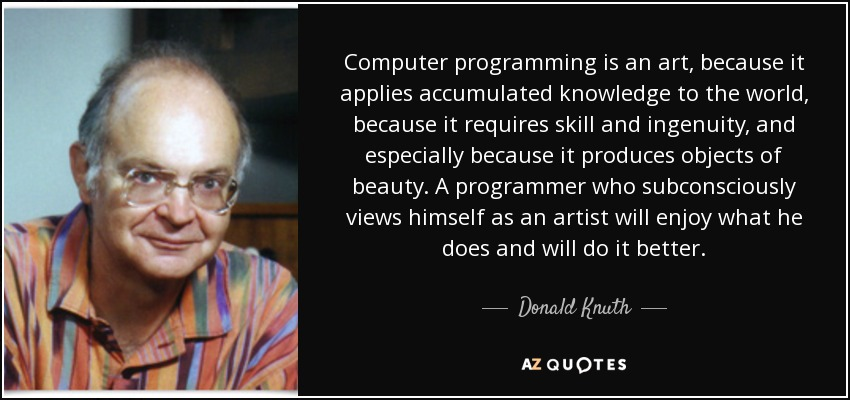
\includegraphics{\path/Knuth.jpg}}
\end{minipage}
\end{center}
\caption{{\TeX}系统的发明人Donald Kunth教授。}
\label{fig_Knuth}
\end{figure}





